\vspace{-2mm}
\section{\sysname{} Overview} \label{sec:design}

Figure~\ref{fig:architecture} depicts the architecture of \sysname{}, which consists of three major components: 
\textit{Hybrid Programming Model}, \textit{3D-HybridEngine} and \textit{Auto-Mapping algorithm}.
The hybrid programming model includes a set of hierarchical APIs to enable flexible expression of the RLHF dataflow and efficient computation of models in the dataflow (\textsection\ref{sec:programming_model}). The 3D-HybridEngine is particularly designed for efficient training and generation of the actor model, allowing different 3D parallel configurations 
in the two stages and %
enabling zero memory redundancy and minimized communication overhead during the transition between two stages (\textsection\ref{sec:hybrid_engine}).
The auto- mapping algorithm determines optimized device %
placement of each model to maximize the throughput of RLHF (\textsection\ref{sec:auto_mapping}).





\begin{figure}[t]
    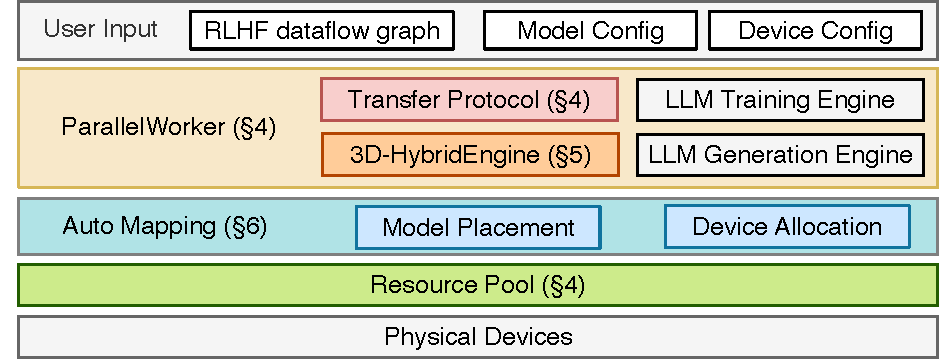
\includegraphics[width=\linewidth]{figs/fig_architecture.pdf}
    \vspace{-5mm}
    \caption{Architecture of HybridFlow. 
    }
    \vspace{-6mm}
    \label{fig:architecture}
\end{figure}


The workflow of our RLHF system goes as follows. A user provides the following inputs to start the RLHF system: (i) model specifications, including
{the architecture and size}
of the actor/critic/reference policy/reward models in the RLHF dataflow;
(ii) device placement of the models in the dataflow, as obtained by running the auto-mapping algorithm under given GPU cluster configurations; (iii) parallelism strategy for running each model in each stage, e.g., a tuple of (p, t, d) for 3D parallelism, where p, t, d represent PP size, TP size and DP size, respectively. %
The single controller program takes these inputs to initialize models in the RLHF dataflow and virtualized resource pool, dispatches operations/models to devices according to the placement plan, and invokes functions run by the multiple controllers on devices to carry out distributed computation of each model.

The multi-controller program implements the ParallelWorker class: it %
constructs parallel groups of each model among allocated devices %
according to its parallelism strategies, 
invokes the 3D-HybridEngine for actor training and generation, and can be integrated seamlessly with existing LLM engines~\cite{shoeybi2019megatron, rasley2020deepspeed, paszke2019pytorch, kwon2023efficient} for training, inference and generation of other models.
The transfer protocols are coordinated by the single controller program to support resharding of data (including prompts, responses, and other model outputs in RLHF) between models with distinct parallelism strategies. The data resharding of the actor between training and generation is handled by 3D-HybridEngine.



